\section{CRC cards}\label{sec:crccards}
In base al colloquio col cliente, possiamo già fornire una prima specifica delle
schede CRC presentate in Tabella \vref{tab:crcc}.
\begin{table}
\begin{center}
\begin{CRCcard}{Reparto}{ }{ }

\end{CRCcard}
\begin{CRCcard}{Referto}{ }{ }

\end{CRCcard}
\end{center}
\begin{center}
\begin{CRCcard}{Prenotazione}{ }{ }

\end{CRCcard}
\begin{CRCcard}{Sala}{ }{ }

\end{CRCcard}
\end{center}
\begin{center}
\begin{CRCcard}{Paziente}{ }{Paziente Minorenne, Paziente Maggiorenne}
\rcline{Autentica}{}
\rcline{Registra}{}
\end{CRCcard}
\end{center}
\begin{center}
\begin{CRCcard}{Amministratore}{}{}
\rcline{Crea Prenotazione}{Paziente, Prenotazione, Reparto, Sala, Messaggio}
\end{CRCcard}
\end{center}
\begin{center}
\begin{CRCcard}{Messaggio}{ }{ }

\end{CRCcard}
\begin{CRCcard}{Paziente Minorenne}{Paziente}{}
\rcline{Registra Tutore}{Tutore}
\rcline{Autentica}{Tutore}
\end{CRCcard}
\end{center}
\begin{center}
\begin{CRCcard}{Paziente Maggiorenne}{}{}
\rcline{Prenota}{Amministratore}
\rcline{Visualizza Storico}{Prenotazione}
\rcline{Visualizza Referto}{Referto}
\rcline{Stampa Storico}{Prenotazione}
\rcline{Stampa Referto}{Referto}
\rcline{Informa amministratore}{Messaggio, Amministratore}
\end{CRCcard}
\end{center}
\begin{center}
\begin{CRCcard}{Tutore}{}{}
\rcline{Prenota}{Paziente Minorenne, Amministratore}
\rcline{Visualizza Storico}{Prenotazione, Paziente Minorenne}
\rcline{Visualizza Referto}{Referto, Paziente Minorenne}
\rcline{Stampa Storico}{Prenotazione, Paziente Minorenne}
\rcline{Stampa Referto}{Referto, Paziente Minorenne}
\rcline{Informa amministratore}{Messaggio, Amministratore}
\end{CRCcard}
\end{center}
\caption{\textit{CRC Cards}.}
\label{tab:crcc}
\end{table}

\section{Modello di dominio}\label{sec:domainmodel}
\begin{figure}[!h]
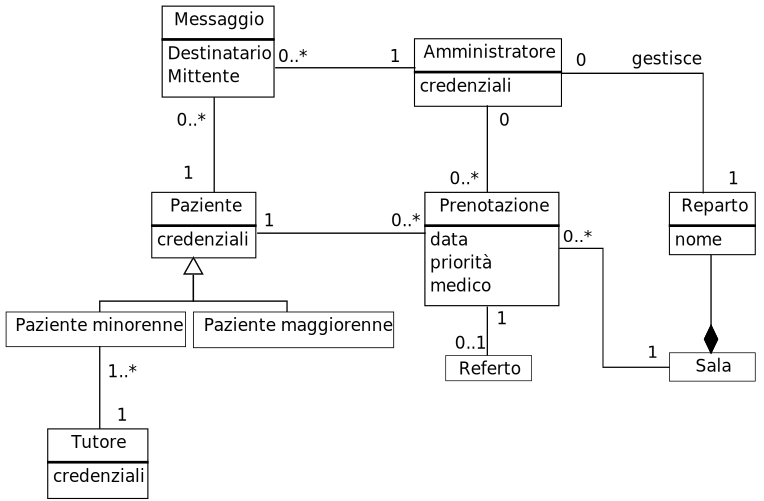
\includegraphics[scale=0.65]{svgs/dominio}
\caption{\textit{Domain Model}.}
\label{fig:dmmdd}
\end{figure}
In seguito ad un primo sviluppo delle schede CRC, possiamo ottenere il modello di
dominio presentato in Figura \vref{fig:dmmdd}.
